\documentclass[10pt,a4paper]{article}

\usepackage[margin=15mm,top=14mm,bottom=15mm]{geometry}
\usepackage[T1]{fontenc}
\usepackage{lmodern}
\usepackage{microtype}
\usepackage{amsmath,amssymb}
\usepackage{booktabs,tabularx,array}
\usepackage{graphicx}
\usepackage{siunitx}
\usepackage{xcolor}
\usepackage{caption}
\usepackage{float}
\usepackage{enumitem}
\usepackage{listings}
\usepackage[backend=biber,style=numeric-comp,sorting=none]{biblatex}
\addbibresource{refs.bib}
\usepackage{xurl}
\usepackage{hyperref}
\usepackage{titlesec}

\definecolor{accent}{HTML}{1F4E79}
\definecolor{lightgray}{HTML}{ECECEC}
\definecolor{codegray}{HTML}{F4F5F6}
\hypersetup{colorlinks=true,linkcolor=accent,citecolor=accent,urlcolor=accent}
\setlength{\parindent}{0pt}
\setlength{\parskip}{3pt}
\setlist[itemize]{nosep,leftmargin=1.4em}
\captionsetup{font=small,labelfont=bf}
\titleformat{\section}{\large\bfseries\color{accent}}{\thesection}{0.6em}{}
\titleformat{\subsection}{\normalsize\bfseries}{\thesubsection}{0.5em}{}
\titlespacing*{\section}{0pt}{7pt}{3pt}
\titlespacing*{\subsection}{0pt}{5pt}{2pt}
\sisetup{per-mode=symbol,detect-all}

\lstdefinestyle{moose}{
  basicstyle=\ttfamily\footnotesize,
  backgroundcolor=\color{codegray},
  frame=single,
  rulecolor=\color{lightgray},
  breaklines=true,
  columns=fullflexible,
  keepspaces=true,
  showstringspaces=false,
  xleftmargin=2mm,
  xrightmargin=2mm,
  aboveskip=4pt,
  belowskip=4pt
}

\begin{document}

{\Large\bfseries\color{accent} EBR-II SHRT-17 XX09 Protected Loss-of-Flow Transient Study}\\[-1mm]
{\large MOOSE/SubChannel -- Part B}\\[2mm]
{\bfseries Omkar Vijay Dhavale}\hfill Independent portfolio study\\
MSc Mechanical Engineering -- Energy, Flow \& Process Technology, TU Delft\hfill 2 October 2026

\vspace{2mm}
\colorbox{lightgray}{\parbox{0.975\linewidth}{\small
\textbf{Study aim.} Extend the Part A steady-state XX09 study to the 900 s SHRT-17 protected loss-of-flow transient, reproduce the public MOOSE/SubChannel calculation with the current upgraded Cheng--Todreas closure, examine the imposed power and flow histories, and compare the predicted TTC-31 temperature response with published experimental measurements digitized from the official MOOSE validation figure.}}

\section{Benchmark and transient scope}

SHRT-17 is an EBR-II shutdown-heat-removal experiment initiated from full-power operation as a protected loss-of-flow event. The benchmark specification documents the initial conditions, pump coastdown, reactor-power history, instrumentation, and quantities used for code comparison \parencite{sumner2012}. Part A of this portfolio established the pre-transient XX09 subassembly operating point. Part B keeps the same local subchannel representation and follows its thermal response through the subsequent 900 s transient.

This is not a full-plant EBR-II calculation. In the public standalone SubChannel validation problem, the XX09 mass-flow and power histories are imposed as functions of time \parencite{moose_ebrii}. The calculation therefore evaluates the bundle-scale thermal response to benchmark forcing; it does not independently predict the system-level pump coastdown or natural-circulation mass flow.

\begin{table}[H]
\centering\small
\caption{Principal transient-model settings used in the present calculation.}
\begin{tabularx}{0.95\linewidth}{@{}lX@{}}
\toprule
Item & Configuration \\
\midrule
Application / problem & MOOSE \texttt{SubChannelApp}; \texttt{TriSubChannel1PhaseProblem} \\
MOOSE package & 2026.09.25 \\
Fluid properties & \texttt{PBSodiumFluidProperties} \parencite{moose_pbsodium} \\
Axial discretization & 50 cells \\
Friction closure & \texttt{SCMFrictionUpgradedChengTodreas} \parencite{moose_ct} \\
Heat-transfer closure & Gnielinski \parencite{gnielinski1975} \\
Mixing closure & Cheng--Todreas, $C_T=2.6$ \\
Transient interval & $t=-1$ to \SI{900}{s}; adaptive time stepping; $\Delta t_{\max}=\SI{20}{s}$ \\
Outlet pressure / inlet temperature & \SI{200}{kPa} / \SI{624.7}{K} \\
Initial XX09 power / mass flow & \SI{486.2}{kW} / \SI{2.45}{kg/s} \\
\bottomrule
\end{tabularx}
\end{table}

\section{Numerical setup, provenance, and execution}

The public MOOSE SHRT-17 transient input was used as the numerical starting point \parencite{moose_ebrii}. Unlike the older software snapshot used in Part A, the MOOSE 2026.09.25 environment accepted the upstream \texttt{SCMFrictionUpgradedChengTodreas} object directly, so no friction-closure substitution was required in the final Part B production case. The original fluid, friction, heat-transfer, mixing, geometry, power, and inlet-flow definitions were retained.

For the production run, only the \texttt{MultiApps} and \texttt{Transfers} blocks used to project the solution onto a separate detailed visualization mesh were removed. This reduced computational overhead without altering the parent SubChannel equations or the prescribed transient forcing. The run reached \SI{900}{s} in 91 adaptive timesteps and completed successfully. One initialization warning reported the bulk Reynolds number outside the upgraded Cheng--Todreas correlation data range at Step 0; no repeated warning was reported during the subsequent transient.

\begin{lstlisting}[style=moose,caption={Core transient time-stepping settings retained from the public validation input.}]
[Executioner]
  type = Transient
  start_time = -1.0
  end_time = 900.0
  [TimeStepper]
    type = IterationAdaptiveDT
    dt = 0.1
    iteration_window = 5
    optimal_iterations = 6
    growth_factor = 1.1
    cutback_factor = 0.8
    timestep_limiting_function = 'time_step_limiting'
  []
  dtmax = 20
[]
\end{lstlisting}

\section{Transient forcing and physical sequence}

The imposed reactor-power history falls much faster than the assembly flow immediately after the transient begins. Power decreases from \SI{486.2}{kW} at $t=0$ to approximately \SI{96.4}{kW} at \SI{1}{s}, while mass flow remains about \SI{2.26}{kg/s}. During the following pump coastdown, however, the flow becomes very small: interpolation of the prescribed history gives approximately \SI{0.0536}{kg/s} at \SI{60}{s}. By then decay power is still approximately \SI{18.6}{kW}. The normalized histories in Fig.~\ref{fig:forcing} make this changing balance between heat generation and coolant transport explicit.

\begin{figure}[H]
\centering
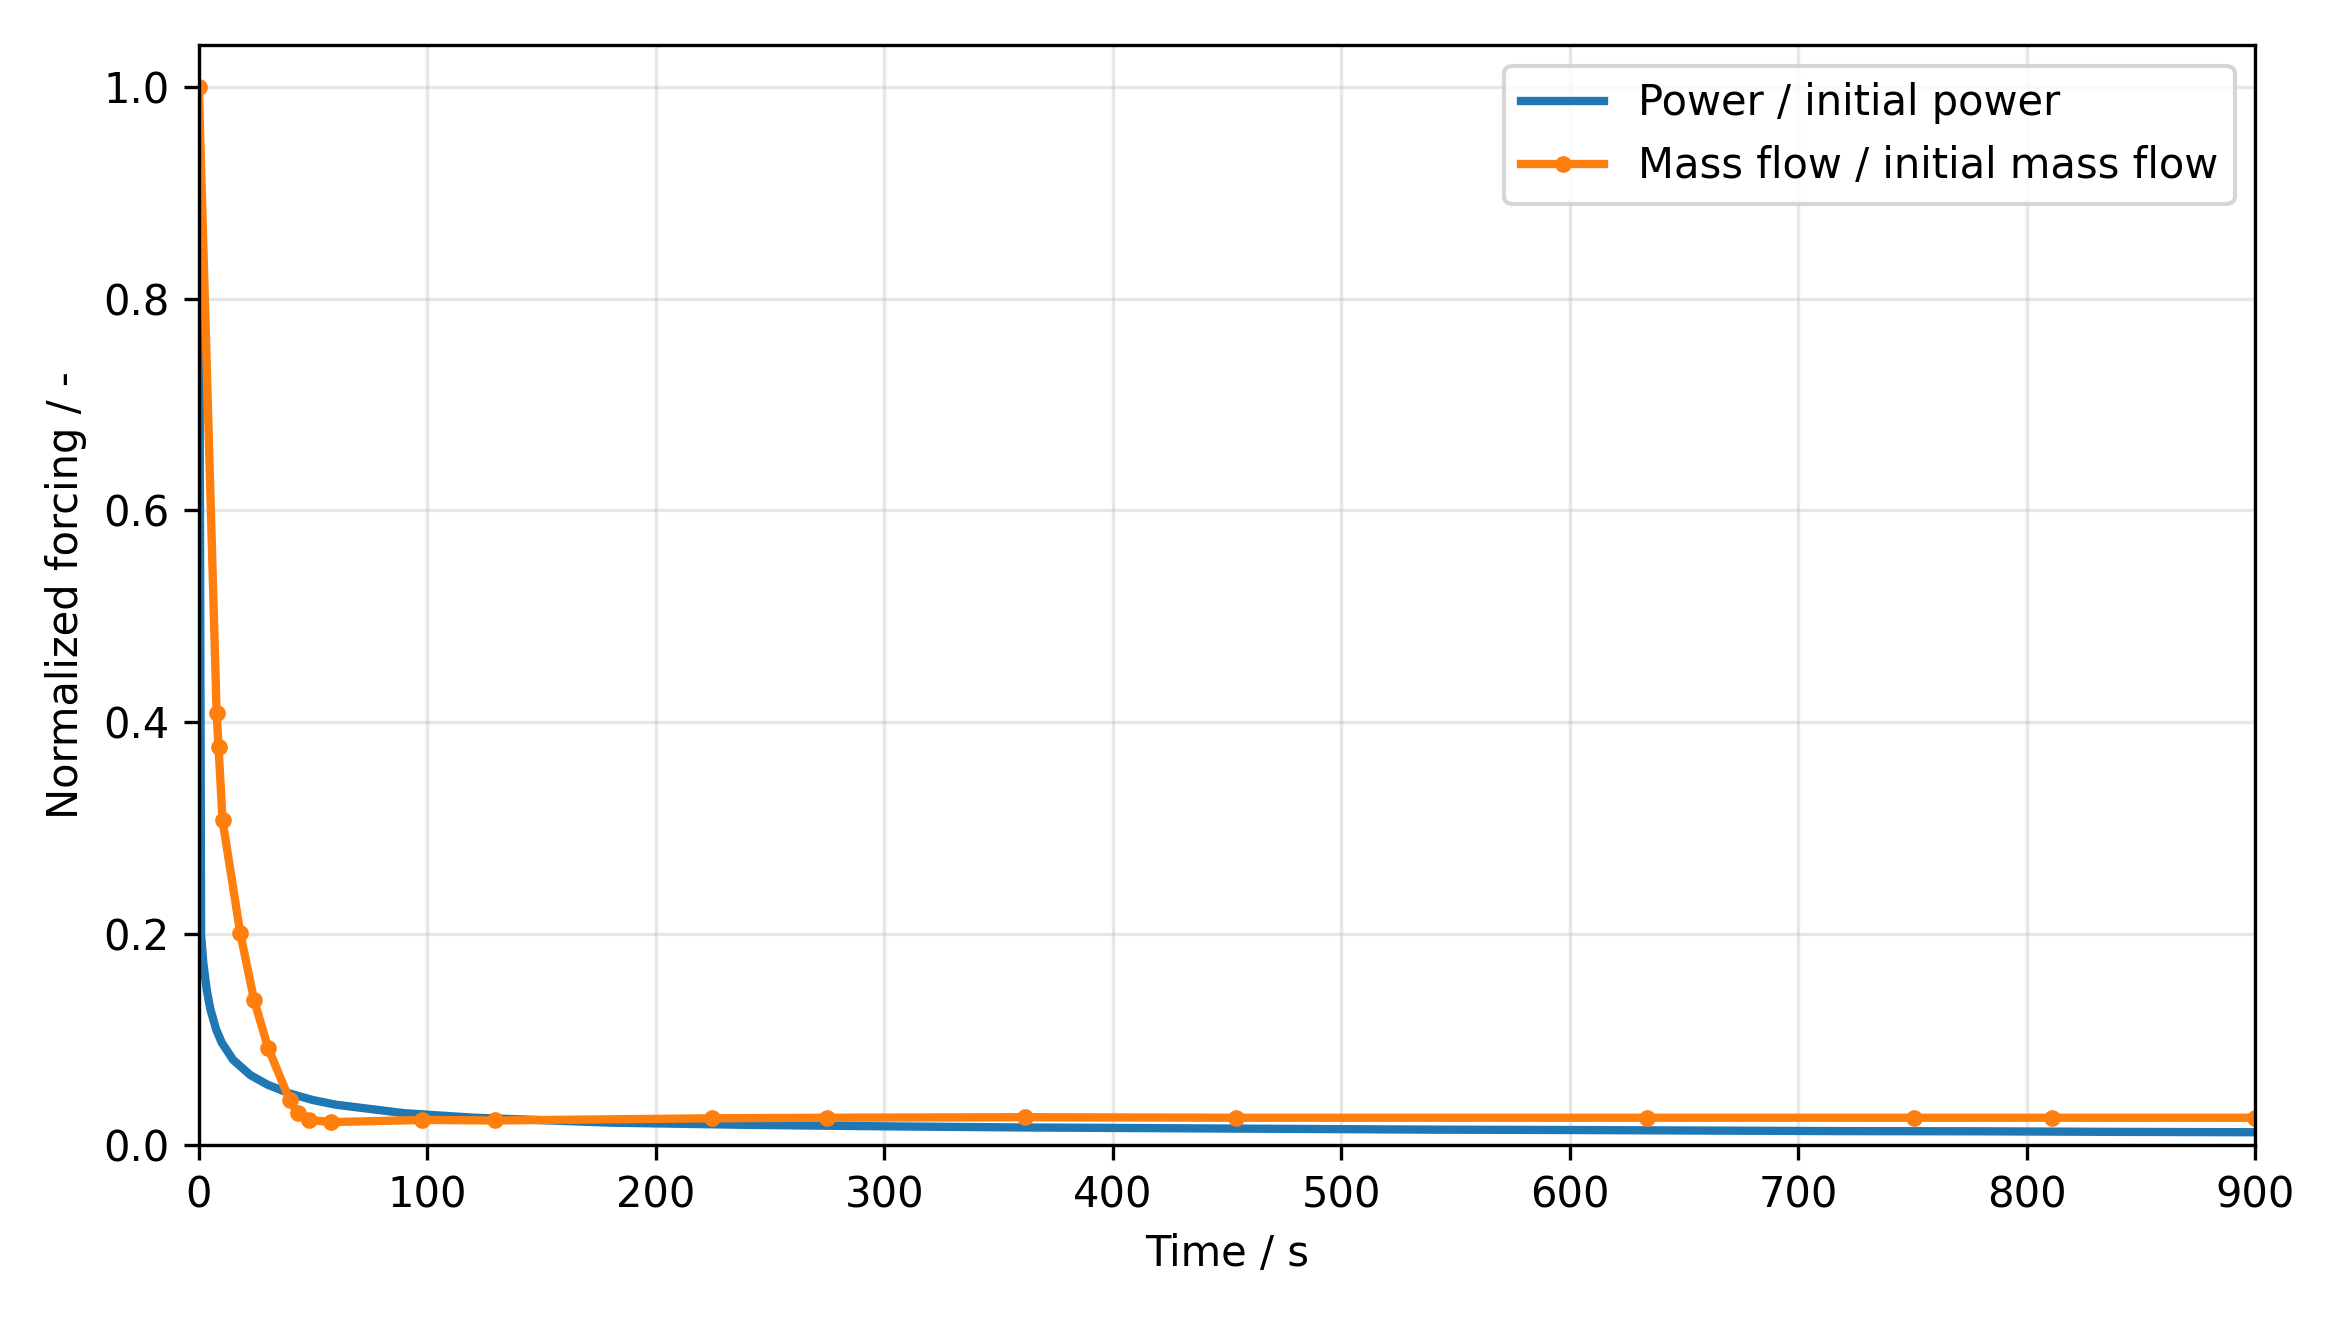
\includegraphics[width=0.78\linewidth]{figures/SHRT17_transient_forcing.png}
\caption{Prescribed SHRT-17 power and XX09 mass-flow histories used in the standalone SubChannel transient. Both quantities are normalized by their initial values.}
\label{fig:forcing}
\end{figure}

A compact way to interpret the sequence is the instantaneous power-to-flow ratio, $\dot Q/\dot m$. It falls from about \SI{198.4}{kJ/kg} initially to \SI{42.6}{kJ/kg} at \SI{1}{s}, consistent with the rapid early coolant cooling. By \SI{60}{s}, the same ratio has risen to approximately \SI{346.5}{kJ/kg} because the mass flow has collapsed more strongly than the remaining decay power. This helps explain the subsequent reheating of TTC-31 before the long-term cooling phase.

\begin{table}[H]
\centering\small
\caption{Selected values from the prescribed forcing histories. Mass flow is linearly interpolated from the public history file.}
\begin{tabular}{@{}rrrrr@{}}
\toprule
$t$ [s] & Power [kW] & $\dot m$ [kg/s] & $\dot m/\dot m_0$ & $\dot Q/\dot m$ [kJ/kg] \\
\midrule
0   & 486.20 & 2.4500 & 1.0000 & 198.45 \\
1   & 96.41  & 2.2638 & 0.9240 & 42.59 \\
10  & 47.19  & 0.7888 & 0.3220 & 59.82 \\
30  & 27.84  & 0.2309 & 0.0942 & 120.58 \\
60  & 18.59  & 0.0536 & 0.0219 & 346.54 \\
300 & 8.66   & 0.0639 & 0.0261 & 135.47 \\
900 & 5.94   & 0.0635 & 0.0259 & 93.51 \\
\bottomrule
\end{tabular}
\end{table}

\section{TTC-31 transient response and experimental comparison}

The final pre-transient output sample gives TTC-31 = \SI{813.54}{K} at $t=-\SI{0.051}{s}$. After the scram, the calculated temperature decreases rapidly to \SI{660.25}{K} at \SI{3.56}{s}. Continued flow coastdown then reduces heat removal enough for TTC-31 to reheat, reaching a calculated maximum of \SI{883.09}{K} at \SI{64.26}{s}. Thereafter the temperature decreases gradually with the continuing decay-power reduction, ending at \SI{696.57}{K} at \SI{900}{s}.

For comparison, the experimental TTC-31 markers were digitized from the official MOOSE SHRT-17 validation figure \parencite{moose_ebrii}. They are therefore treated as figure-derived values rather than raw experimental data. The digitized experimental peak is approximately \SI{892.12}{K} at \SI{74.0}{s}. Relative to that point, the present MOOSE calculation predicts the peak \SI{9.03}{K} lower and \SI{9.74}{s} earlier.

\begin{figure}[H]
\centering
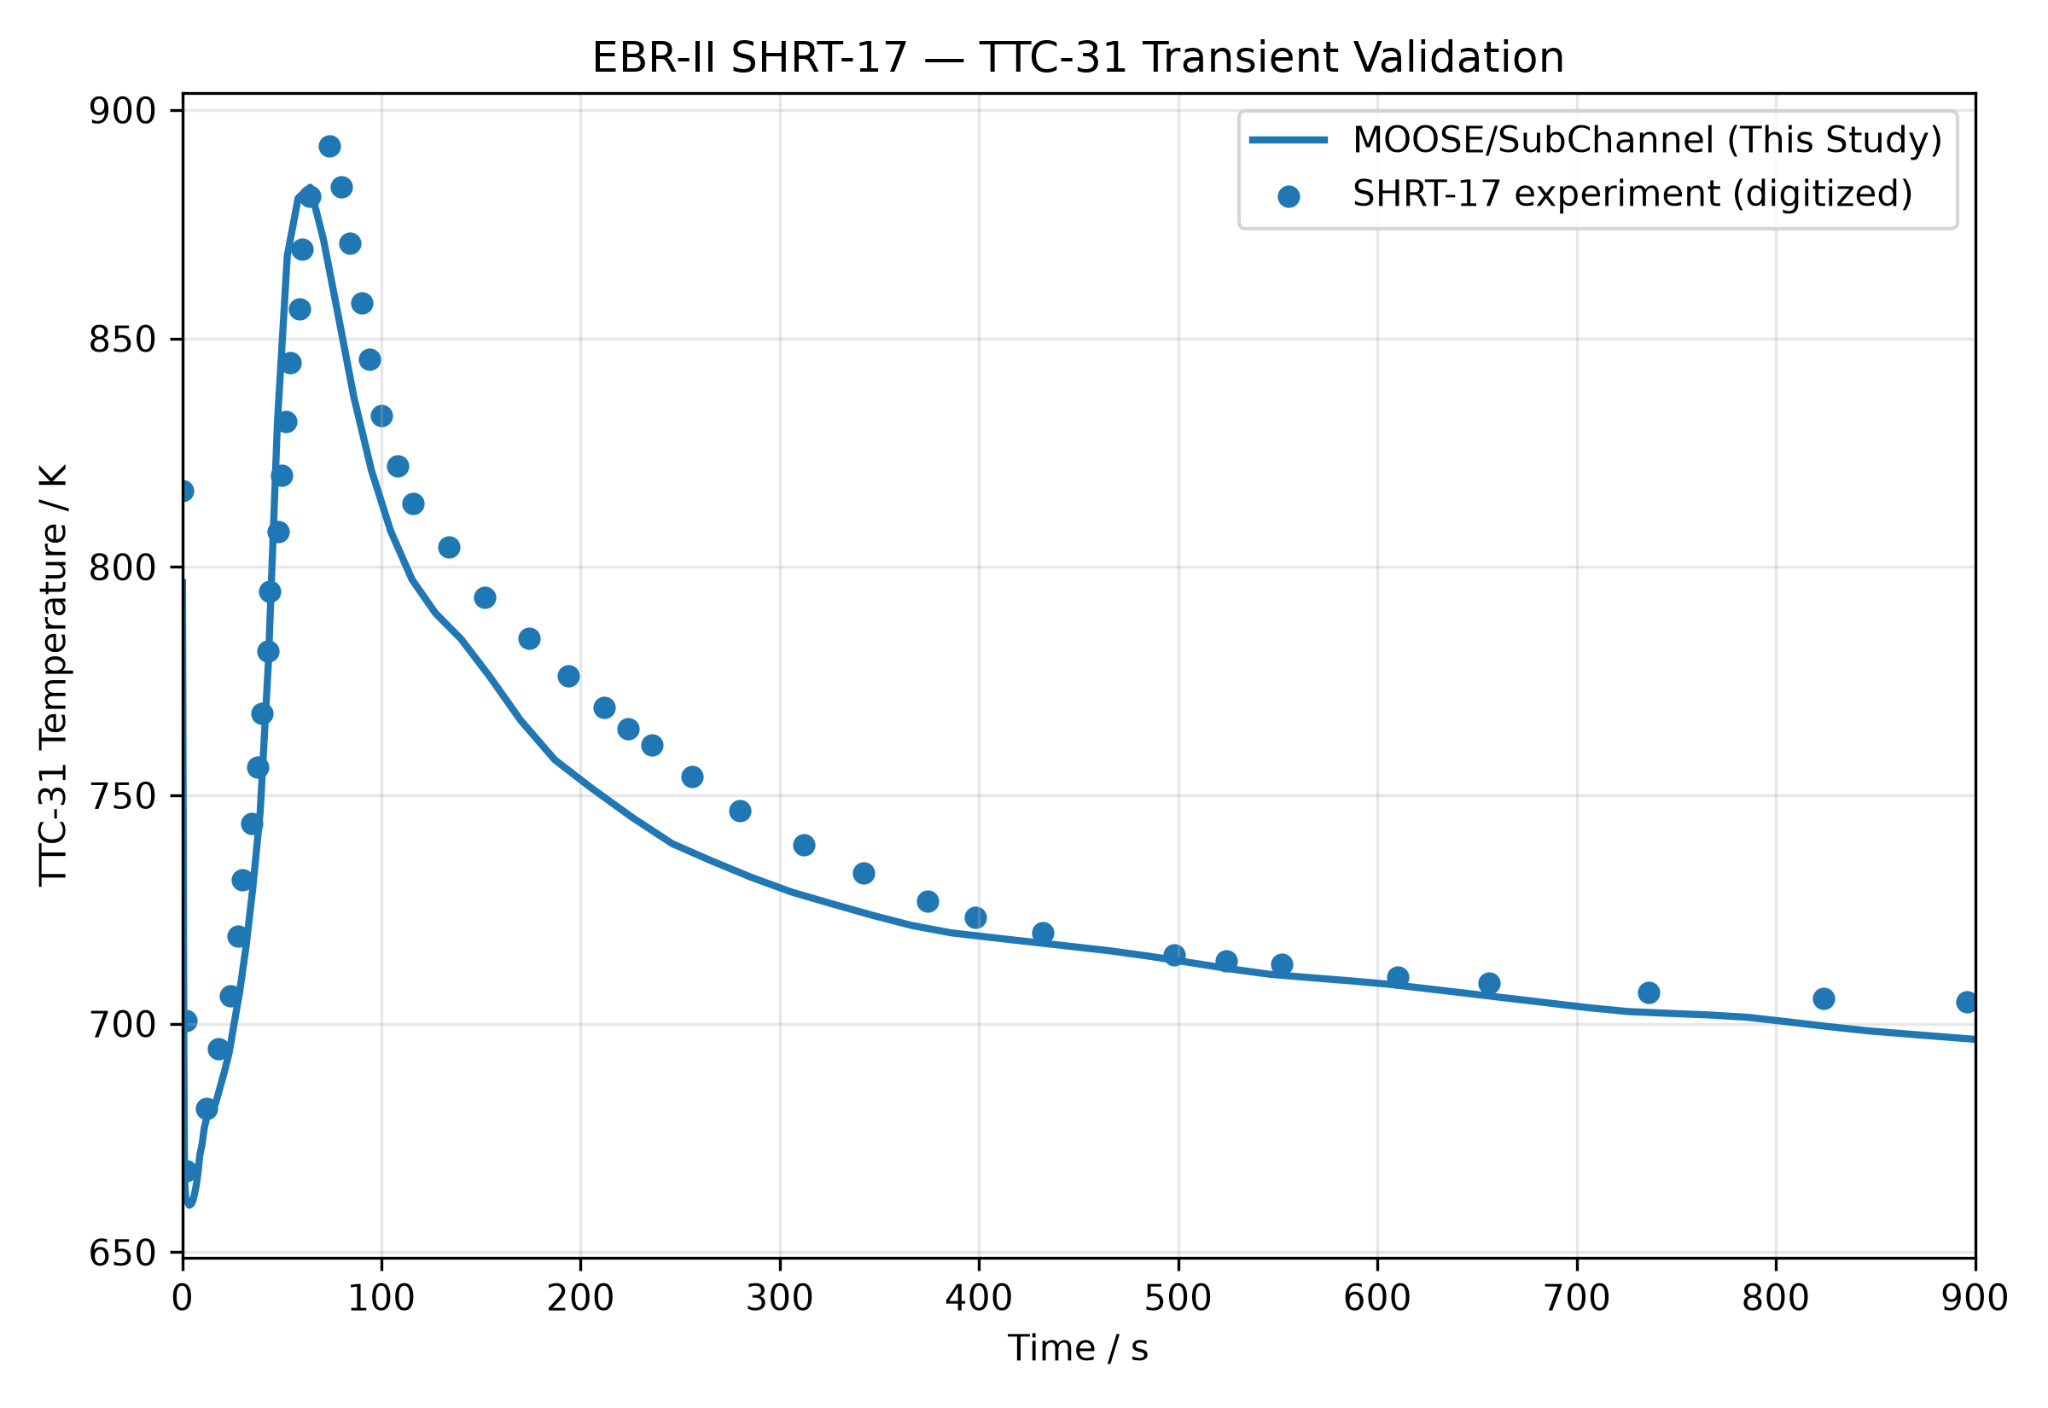
\includegraphics[width=0.94\linewidth]{figures/SHRT17_TTC31_validation.png}
\caption{TTC-31 transient temperature from the present MOOSE/SubChannel run and experimental markers digitized from the published MOOSE SHRT-17 validation figure \parencite{moose_ebrii}.}
\label{fig:ttc}
\end{figure}

The simulation was interpolated to the 50 digitized experimental measurement times. For paired values $T_i^{\mathrm{M}}$ and $T_i^{\mathrm{E}}$, the reported summary errors are
\begin{equation}
\mathrm{MAE}=\frac{1}{N}\sum_{i=1}^{N}\left|T_i^{\mathrm{M}}-T_i^{\mathrm{E}}\right|,
\qquad
\mathrm{RMSE}=\sqrt{\frac{1}{N}\sum_{i=1}^{N}\left(T_i^{\mathrm{M}}-T_i^{\mathrm{E}}\right)^2}.
\end{equation}
The resulting values are MAE = \SI{14.88}{K} and RMSE = \SI{17.65}{K}. The calculation reproduces the main qualitative sequence and the long cooling tail, while the predicted transient peak is somewhat lower and earlier than the digitized measurement peak.

\begin{table}[H]
\centering\small
\caption{Headline TTC-31 transient comparison.}
\begin{tabular}{@{}lr@{}}
\toprule
Quantity & Result \\
\midrule
Pre-transient TTC-31 & \SI{813.54}{K} \\
Post-scram minimum & \SI{660.25}{K} at \SI{3.56}{s} \\
MOOSE peak & \SI{883.09}{K} at \SI{64.26}{s} \\
Digitized experimental peak & \SI{892.12}{K} at \SI{74.0}{s} \\
Peak-temperature difference & \SI{-9.03}{K} \\
Peak-time difference & \SI{-9.74}{s} \\
MAE / RMSE & \SI{14.88}{K} / \SI{17.65}{K} \\
Final TTC-31 at 900 s & \SI{696.57}{K} \\
\bottomrule
\end{tabular}
\end{table}

\section{Interpretation, limitations, and conclusions}

Part B reproduces the public SHRT-17 XX09 transient with the current upgraded Cheng--Todreas friction closure and provides a transparent code-to-data check of TTC-31. The calculated temperature exhibits the expected three-stage behavior: a rapid post-scram decrease as power collapses, reheating as the imposed flow coastdown becomes dominant, and a long decay-heat cooling tail. The predicted peak is about \SI{1.0}{\percent} below the digitized experimental peak and occurs about \SI{9.7}{s} earlier; the full set of digitized points gives MAE = \SI{14.88}{K} and RMSE = \SI{17.65}{K}.

The result should be interpreted within the model scope. The standalone XX09 calculation uses prescribed power and mass-flow histories, so it does not constitute an independent system-level prediction of pump coastdown or natural circulation. The comparison data were digitized from a published figure, not obtained from the original measurement file, and therefore include small digitization uncertainty. The calculation also represents one instrumented subassembly rather than the full EBR-II primary system. These limitations make the study suitable as a reproducible portfolio validation exercise, not as a licensing-grade safety analysis.

\vspace{1mm}
{\small\textbf{Provenance statement.} Argonne provides the SHRT-17 benchmark specification \parencite{sumner2012}; the MOOSE project provides the public XX09 transient validation setup and published comparison figure \parencite{moose_ebrii}. For this study, the transient was executed in MOOSE 2026.09.25, the visualization-only MultiApp/transfer blocks were removed from the production input, transient quantities were extracted and interpreted, the published TTC-31 measurements were digitized, error metrics were calculated, and the figures and technical note were produced independently.}

\printbibliography[title={References}]

\end{document}
